\documentclass[10.5pt,compsoc,UTF8]{CjC}
\usepackage{CTEX}
\usepackage{graphicx}
\usepackage{footmisc}
\usepackage{subfigure}
\usepackage{url}
\usepackage{multirow}
\usepackage{multicol}
\usepackage[noadjust]{cite}
\usepackage{amsmath,amsthm}
\usepackage{amssymb,amsfonts}
\usepackage{booktabs}
\usepackage{color}
\usepackage{ccaption}
\usepackage{booktabs}
\usepackage{float}
\usepackage{fancyhdr}
\usepackage{caption}
\usepackage{xcolor,stfloats}
\usepackage{comment}
\setcounter{page}{1}
\graphicspath{{figures/}}
\usepackage{cuted}
\usepackage{captionhack}
\usepackage{epstopdf}
\usepackage{gbt7714}
\usepackage{stfloats}
\usepackage{amsmath}
\usepackage{arydshln}
%===============================%

%=======设置奇偶页页眉=======%
\headevenname{\mbox{\quad} \hfill  \mbox{\zihao{-5}{计\quad \quad 算\quad \quad 机\quad \quad 学\quad \quad 报} \hspace {50mm} \mbox{2023 年}}}%
\headoddname{? 期 \hfill
作者姓名等:论文题目}
%=======设置奇偶页页眉=======%

\renewcommand{\thefootnote}{\fnsymbol{footnote}}
\setcounter{footnote}{0}
\renewcommand\footnotelayout{\zihao{5-}}
\newtheoremstyle{mystyle}{0pt}{0pt}{\normalfont}{1em}{\bf}{}{1em}{}
\theoremstyle{mystyle}
\renewcommand\figurename{figure~}
\renewcommand{\thesubfigure}{(\alph{subfigure})}
\newcommand{\upcite}[1]{\textsuperscript{~\cite{}}
\renewcommand{\labelenumi}{(\arabic{enumi})}
\newcommand{\tabincell}[2]{\begin{tabular}{@{}#1@{}}#2\end{tabular}}
\newcommand{\abc}{\color{white}\vrule width 2pt}
\renewcommand{\bibsection}{}
\makeatletter
\renewcommand{\@biblabel}[1]{[#1]\hfill}
\makeatother
\setlength\parindent{2em}

\pagestyle{CjCheadings}
\setmainfont{Times New Roman}

%===========================================================%
\begin{document}

\hyphenpenalty=50000
\makeatletter
\newcommand\mysmall{\@setfontsize\mysmall{7}{9.5}}
\newenvironment{tablehere}
  {\def\@captype{table}}

\let\temp\footnote
\renewcommand \footnote[1]{\temp{\zihao{-5}#1}}

%=======设置首页页眉=======%
\thispagestyle{empty}%
\begin{table*}[!t]
\vspace {-13mm}
\onecolumn
\noindent\begin{tabular}{p{168mm}}
\zihao{5-}
第??卷\quad 第?期 \hfill 计\quad 算\quad 机\quad 学\quad 报\hfill Vol. ??  No. ?\\
\zihao{5-}
20??年?月 \hfill CHINESE JOURNAL OF COMPUTERS \hfill ???. 20??\\
\hline\\[-5.5mm]
\hline\end{tabular}\end{table*}
%=======设置首页页眉=======%

%中文标题、作者与注脚
{
\centering
\vspace {11mm}
{\zihao{2} \heiti 题目(中英文题目一致)字体为2号黑体(全文除特别声明外, 外文统一用Times New Roman) }

\vskip 5mm

{\zihao{3}\fangsong 作者名$^{1)}$\quad  作者名$^{2),3)}$ \quad 作者名$^{3) }$($^*$字体为3号仿宋*作者)}
\footnote{\noindent \zihao{6}\songti 收稿日期:\quad \quad -\quad -\quad ;最终修改稿收到日期:\quad \quad -\quad -\quad .*投稿时不填写此项*. 本课题得到… …基金中文完整名称(No.项目号)、… …基金中文完整名称(No.项目号)、… … 基金中文完整名称(No.项目号)资助.\textsf{作者名1(通信作者)},性别,xxxx年生,学位(或目前学历),职称,是/否计算机学会(CCF)会员(提供会员号),主要研究领域为*****、****.E-mail: **************.\textsf{作者名2(通信作者)},性别,xxxx年生,学位(或目前学历),职称,是/否计算机学会(CCF)会员(提供会员号),主要研究领域为*****、****.E-mail: **************. \textsf{作者名3(通信作者)},性别,xxxx年生,学位(或目前学历),职称,是/否计算机学会(CCF)会员(提供会员号),主要研究领域为*****、****.E-mail: **************.(给出的电子邮件地址应不会因出国、毕业、更换工作单位等原因而变动。请给出所有作者的电子邮件)
第1作者手机号码(投稿时必须提供,以便紧急联系,发表时会删除): … …, E-mail: … …*此部分6号宋体*}

\vspace {1mm}

\zihao{6}{$^{1)}$(单位全名 部门(系)全名, 市(或直辖市) 国家名 邮政编码) *字体为6号宋体*单位}

\zihao{6}{$^{2)}$(单位全名 部门(系)全名, 市(或直辖市) 国家名 邮政编码)*中英文单位名称、作者姓名须一致*}

\zihao{6}{$^{3)}$(单位全名 部门(系)全名, 市(或直辖市) 国家名 邮政编码)}

\zihao{6}{\textsf{论文定稿后,作者署名、单位无特殊情况不能变更。若变更,须提交签章申请,国家为中国可以不写,省会城市不写省名,其他国家必须写国家名。}}
}%中文标题、作者与注脚

\vskip 5mm

\zihao{5-}{
\setlength{\baselineskip}{16pt}\selectfont{
\noindent {\heiti 摘\quad 要\quad }
*中文摘要内容置于此处(英文摘要中要有这些内容),字体为小5号宋体。摘要贡献部分,要有数据支持,不要出现``...大大提高''、``...显著改善''等描述,正确的描述是``比{\ldots}提高X{\%}''、``在{\ldots}上改善X{\%}''。*摘要\par}}

\vspace {5mm}

\zihao{5-}{\noindent
{\heiti 关键词 \quad }{*关键词(中文关键字与英文关键字对应且一致,应有5-7个关键词);关键词;关键词;关键词*  }
}\par\noindent
\zihao{5-}{\heiti 中图法分类号\quad } TP\rm{\quad \quad \quad     }
{\heiti DOI号:\quad } *投稿时不提供DOI号

\vskip 5mm

\begin{center}
\zihao{3}{ \heiti Title *(中英文题目一致)字体为4号Times New Roman,加粗* Title}\\
\vspace {5mm}
\zihao{5}{ NAME Name-Name$^{1)}$ NAME Name$^{2)}$ NAME Name-Name$^{3)}$ *字体为5号Times new Roman*Name}\\
\vspace {1mm}
\zihao{6}{{$^{1)}$(Department of ****, University, City ZipCode, China) *字体为6号Times new Roman* Depart.Correspond}}

\zihao{6}{{$^{2)}$(Department of ****, University, City ZipCode)*中国不写国家名*}}

\zihao{6}{{$^{3)}$(Department of ****, University, City ZipCode, country)*外国写国家名*}}

\end{center}

\zihao{5}{
{\noindent\bf Abstract}\quad (\textbf{500英文单词,内容包含中文摘要的内容}).
字体为Times new Roman,字号5号*
\zihao{5}{\noindent Do not modify the amount of space before and after the artworks. One- or two-column format artworks are preferred. and Tables, create a new break line and paste the resized artworks where desired. Do not modify the amount of space before and after the artworks. One- or two-column format artworks are preferred. All Schemes, Equations, Figures, and Tables should be mentioned in the text consecutively and numbered with Arabic numerals, and appear below where they are mentioned for the first time in the main text. To insert Schemes, Equations, Figures, and Tables, create a new break line and paste the resized artworks where desired. Do not modify the amount of space before and after the artworks. One- or two-column format artworks are preferred.Do not modify the amount of space before and after the artworks. One- or two-column format artworks are preferred. and Tables, create a new break line and paste the resized artworks where desired.
\par}}

\vspace {5mm}

\zihao{5}{
{\noindent\bf Keywords}\quad 中文关键字与英文关键字对应且一致,\textbf{不要用英文缩写});
key word; key word; key word* *字体为5号Times new Roman * Key words
\par}

\zihao{5}
\vskip 1mm
\begin{multicols}{1}

\section{\heiti 一级标题*字体为4号黑体*标题1}

这是一个CTEX的utf-8编码例子,{\kaishu 这里是楷体显示},{\songti 这里是宋体显示},{\heiti 这里是黑体显示},{\fangsong 这里是仿宋显示}。另外一种方式:\textit{这是楷体显示,but英文和数字是斜体abcABC123},\textsf{这是黑体显示abcACB123},\texttt{这是仿宋显示abcABC123}。

\subsection{\heiti 关于数学部分}
数学、中英文皆可以混排。You can intersperse math, Chinese and English (Latin script) without adding extra environments.

\subsection{\heiti 对投稿的基本要求}

(1) 研究性论文主体应包括引言(重点论述研究的科学问题、意义、解决思路、价值、贡献等)、相关工作(为与引言部分独立的一个章节)、主要成果论述、关键实现技术、验证(对比实验或理论证明)、结论(结束语)等内容;系统实现或实验应有关键点的详细论述,以便读者能够重复实现论文所述成果。实验应有具体的实验环境设置、全面细致的数据对比分析。

(2) 综述应包括引言、问题与挑战、研究现状分析、未来研究方向、结论等内容。以分析、对比为主,避免堆砌文献或一般性介绍、叙述。

(3) 定理证明、公式推导、大篇幅的数学论述、原始数据,放到论文最后的附录中。

{\bf 稿件提交时的基本要求:}

(1) 本模板中要求的各项内容正确齐全,无遗漏;

(2) 语句通顺,无中文、英文语法错误,易于阅读理解,符号使用正确,图、表清晰无误;

(3) 在学术、技术上,论文内容正确无误,各项内容确定。

{\heiti \subsection{二级标题 *字体为5号黑体*标题2}}
\subsubsection{三级标题 *字体为5号宋体*标题3}
*正文部分, 字体为5号宋体* 正文文字

\textbf{正文文字要求语句通顺,无语法错误,结构合理,条理清楚,不影响审稿人、读者阅读理解全文内容。以下几类问题请作者们特别注意}:

1) 文章题目应明确反映文章的思想和方法;文字流畅,表述清楚;

2) 中文文字、英文表达无语法错误;

3) 公式中无符号、表达式的疏漏,没有同一个符号表示两种意思的情况;

4) 数学中使用的符号、函数名用斜体;

5) 使用的量符合法定计量单位标准;

6) 矢量为黑体,标量为白体;

7) 变量或表示变化的量用斜体;

8) 图表规范,量、线、序无误,位置正确(图表必须在正文中有所表述后出现,即{\ldots}如图1所示)(注意纵、横坐标应有坐标名称和刻度值)。

9) 列出的参考文献必须在文中按顺序引用,即参考文献顺序与引用顺序一致,各项信息齐全(格式见参考文献部分);

10) 首次出现的缩写需写明全称,首次出现的符号需作出解释。

11) 图的图例说明、坐标说明全部用中文或量符号。

\textbf{12) 图应为矢量图。}

13) 表中表头文字采用中文。

14) 公式尺寸:

标准:10.5磅

下标/上标:5.8磅

次下标/上标:4.5磅

符号:16磅

次符号:10.5磅

15) 组合单位采用标准格式,如:``pJ/bit/m$^{4}$''应为 ``pJ/(bit$\cdot
$m$^{4})$''

\textbf{定理1}.\quad ******. *定理内容.*

[``定义''、``假设''、``公理''、``引理''等的排版格式与此相同,详细定理证明、公式可放在附录中]

\texttt{证明}.\quad  *证明过程.* [``例 x''等的排版格式相同]

\rightline {证毕.}

\begin{figure}[H]
\centerline{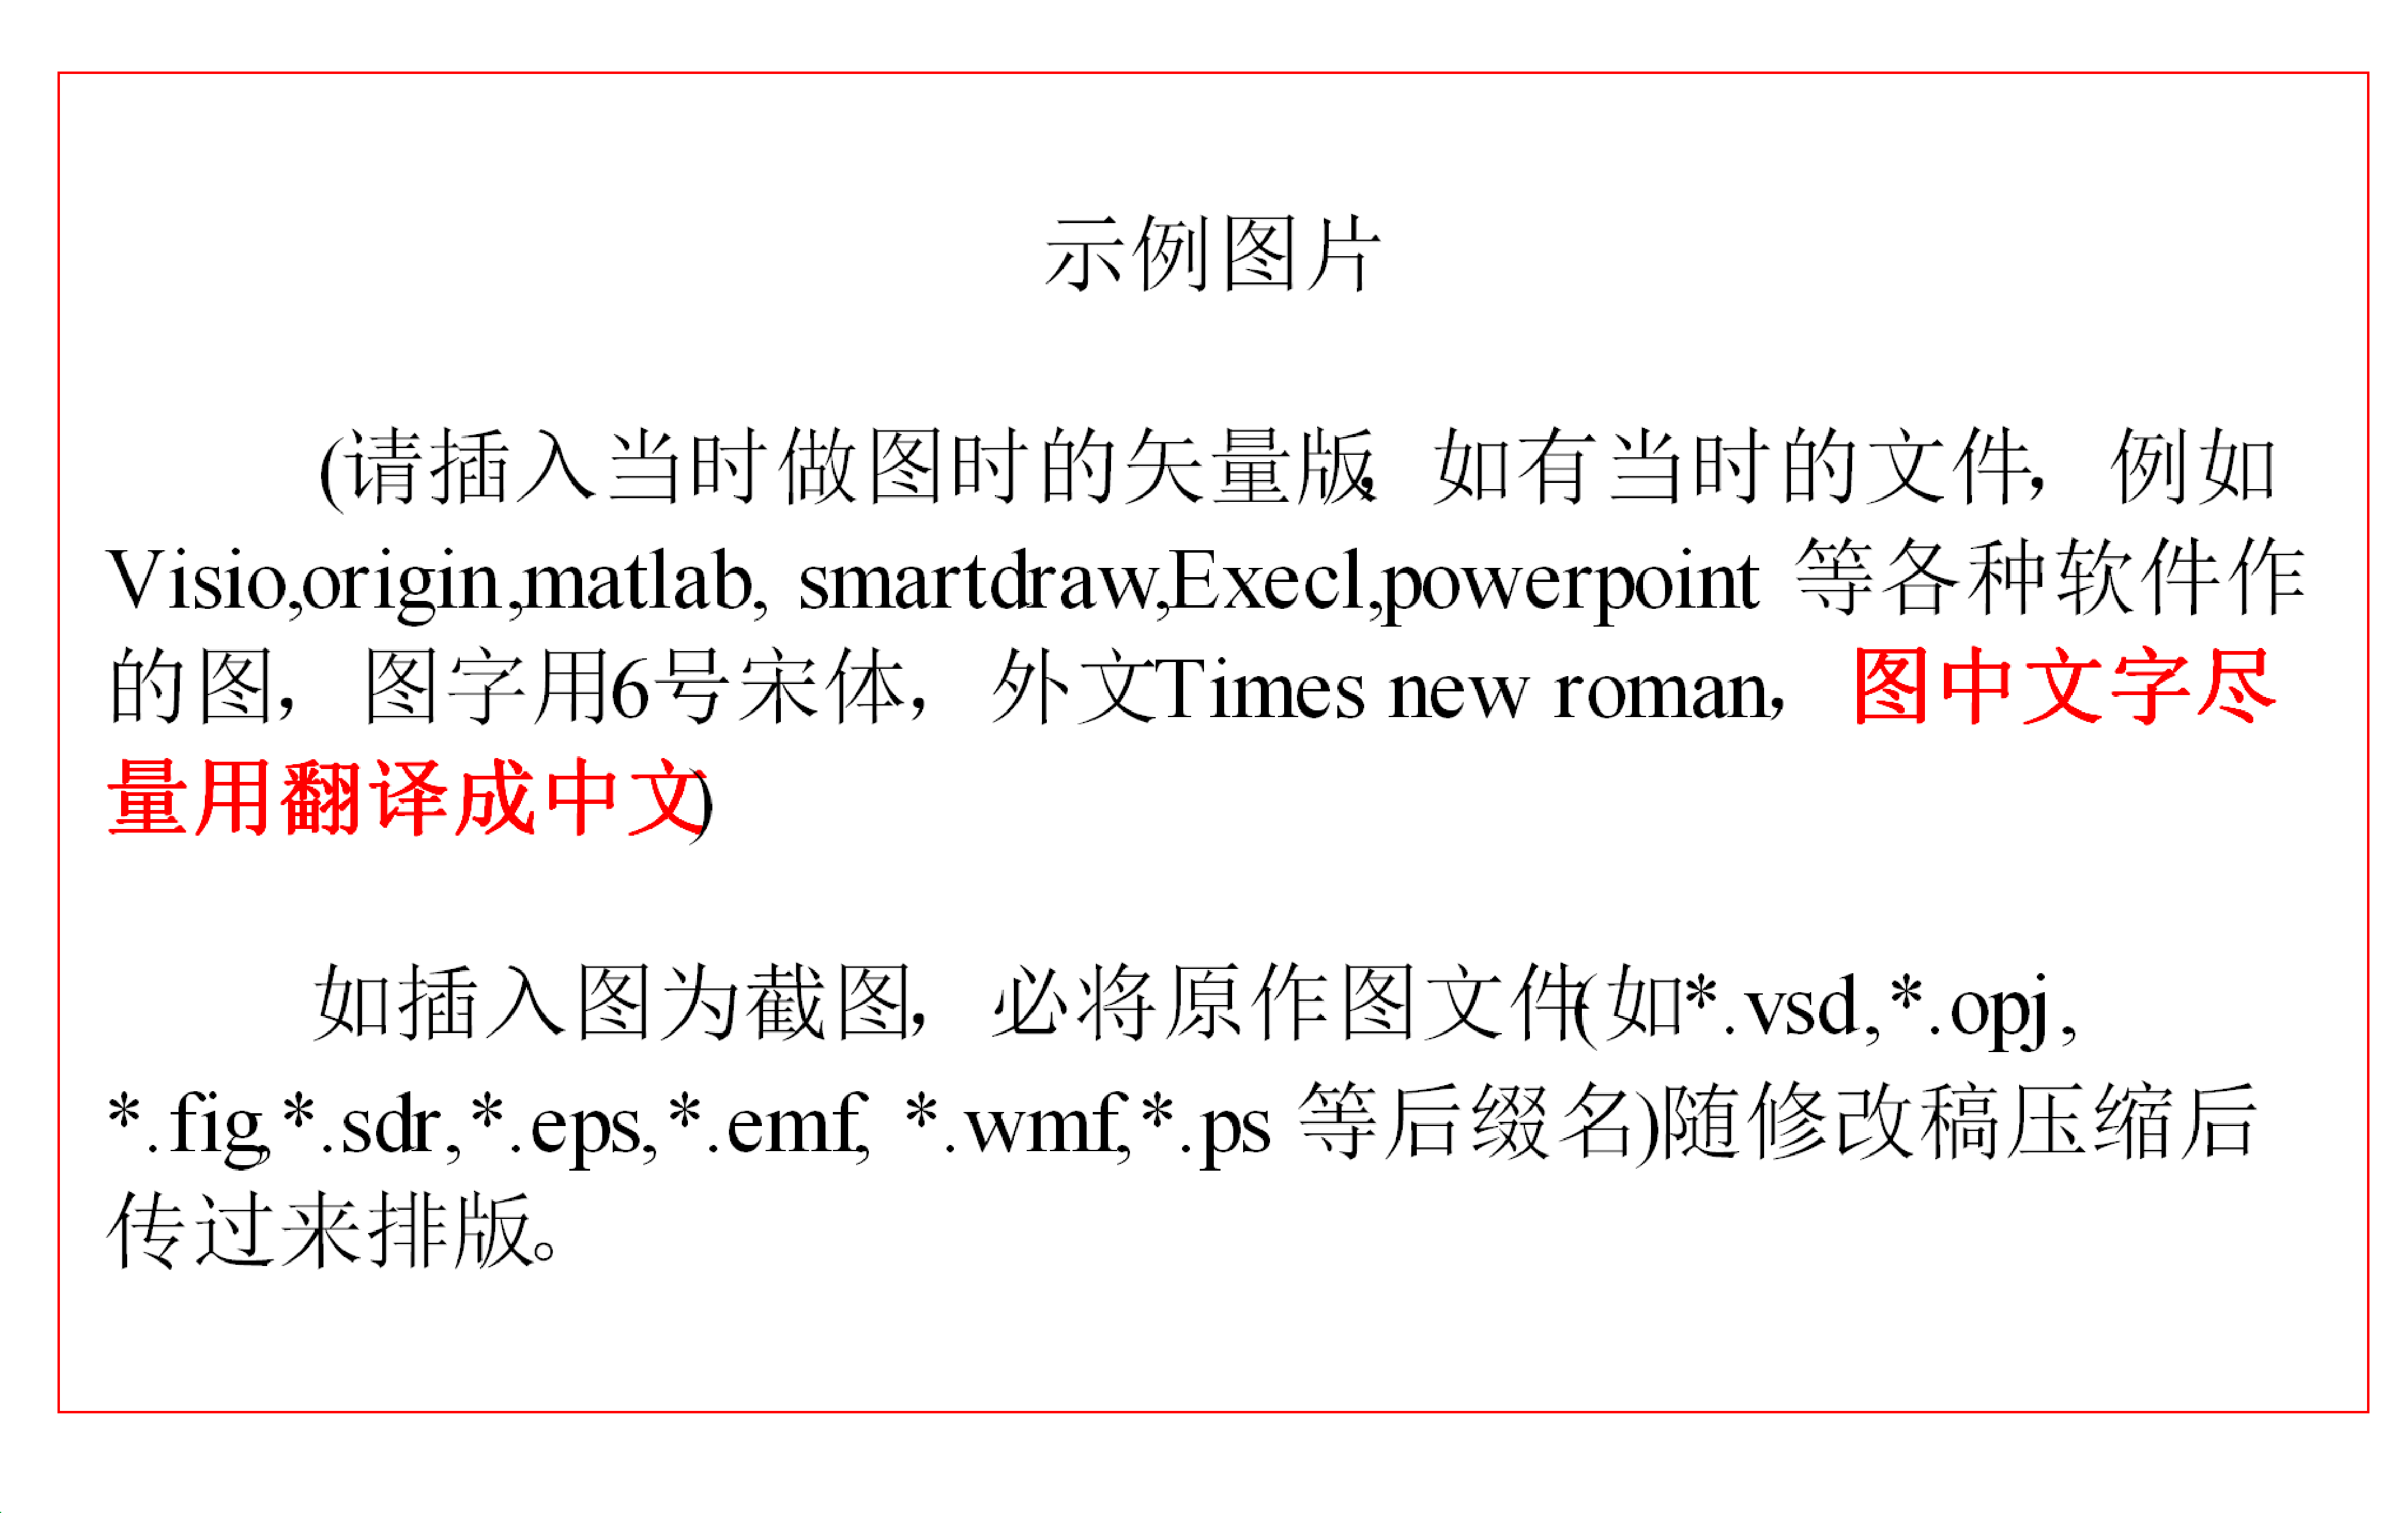
\includegraphics[width=3.15in,height=1.98in]{CJC1.pdf}}
{\zihao{5}图X\quad  图片说明 *字体为小5号,图片应为黑白图,图中的子图要有子图说明*}
\label{fig1}
\end{figure}

\begin{table}[H]
\centering {\heiti 表X\quad 表说明 *表说明采用黑体*}
% \caption{表说明 *表说明采用黑体*}
\vspace {-2.5mm}
\begin{center}
\begin{tabular}{ll}
\toprule
*示例表格*&*第1行为表头,表头要有内容* \\
\hline
&
 \\
&
 \\
&
 \\
&
 \\
\bottomrule
\end{tabular}
\label{tab1}
\end{center}
\end{table}

{\heiti 过程X}.\quad 过程名称

{\zihao{5-}*《计算机学报》的方法过程描述字体为小5号宋体,IF、THEN等伪代码关键词全部用大写字母,变量和函数名称用斜体*}


{\heiti 算法\textbf{Y}}.\quad 算法名称.
{\zihao{5-}

\noindent 输入:{\ldots} {\ldots}

\noindent 输出:{\ldots} {\ldots}

*《计算机学报》的算法描述字体为小5号宋体, IF、THEN等伪代码关键词全部用大写字母,变量和函数名称用斜体*}

\subsubsection{参考文献}
这是参考文献示例。参考文献应遵循GB/T 7741-2015标准。引用文献1~\cite{Bohan1928},文献2~\cite{chen1980zhongguo},文献3-5~\cite{bravo1990comparative,niu2013zonghe,yuan2012lana}。

\vspace {3mm}
\zihao{5}{
\noindent \textsf{致\quad 谢}\quad \textit{ *致谢内容.* 致谢}}

\vspace {5mm}
\centerline
{\zihao{5}\textsf{参~考~文~献}}
\zihao{5-} \addtolength{\itemsep}{-1em}
\vspace {1.5mm}
\bibliographystyle{gbt7714-numerical}
\bibliography{ref.bib}

\end{multicols}

\begin{multicols}{1}
\noindent {\zihao{5}\bf{附录X}.}

{\zihao{5-}\setlength\parindent{2em}
*\textbf{附录内容}置于此处,字体为小5号宋体。附录内容包括:\textbf{详细的定理证明、公式推导、原始数据}等*}\\\\

\end{multicols}


\begin{multicols}{1}
\begin{biography}[yourphotofilename.jpg]
\noindent
\textbf{First A. Author}\ \ *计算机学报第1作者提供照片电子图片,尺寸为1寸。英文作者介绍内容包括:出生年,学位(或目前学历),职称,主要研究领域(\textbf{与中文作者介绍中的研究方向一致}).*
*字体为小5号Times New Roman*
\end{biography}

\begin{biography}[yourphotofilename.jpg]
\noindent
\textbf{Second B. Author} *英文作者介绍内容包括:出生年,学位(或目前学历),职称,主要研究领域(\textbf{与中文作者介绍中的研究方向一致})。*
*字体为小5号Times New Roman*
\end{biography}
\end{multicols}


\begin{multicols}{1}
\zihao{5}
\noindent \textbf{Background}

\zihao{5-}{
\setlength\parindent{2em}
*论文背景介绍为\textbf{英文},字体为小5号Times New Roman体*

论文后面为400单词左右的英文背景介绍。介绍的内容包括:

本文研究的问题属于哪一个领域的什么问题。该类问题目前国际上解决到什么程度。

本文将问题解决到什么程度。

课题所属的项目。

项目的意义。

本研究群体以往在这个方向上的研究成果。

本文的成果是解决大课题中的哪一部分,如果涉及863$\backslash
$973以及其项目、基金、研究计划,注意这些项目的英文名称应书写正确。}

\end{multicols}
\end{document}
